% Created by tikzDevice version 0.12.6 on 2025-02-04 13:53:20
% !TEX encoding = UTF-8 Unicode
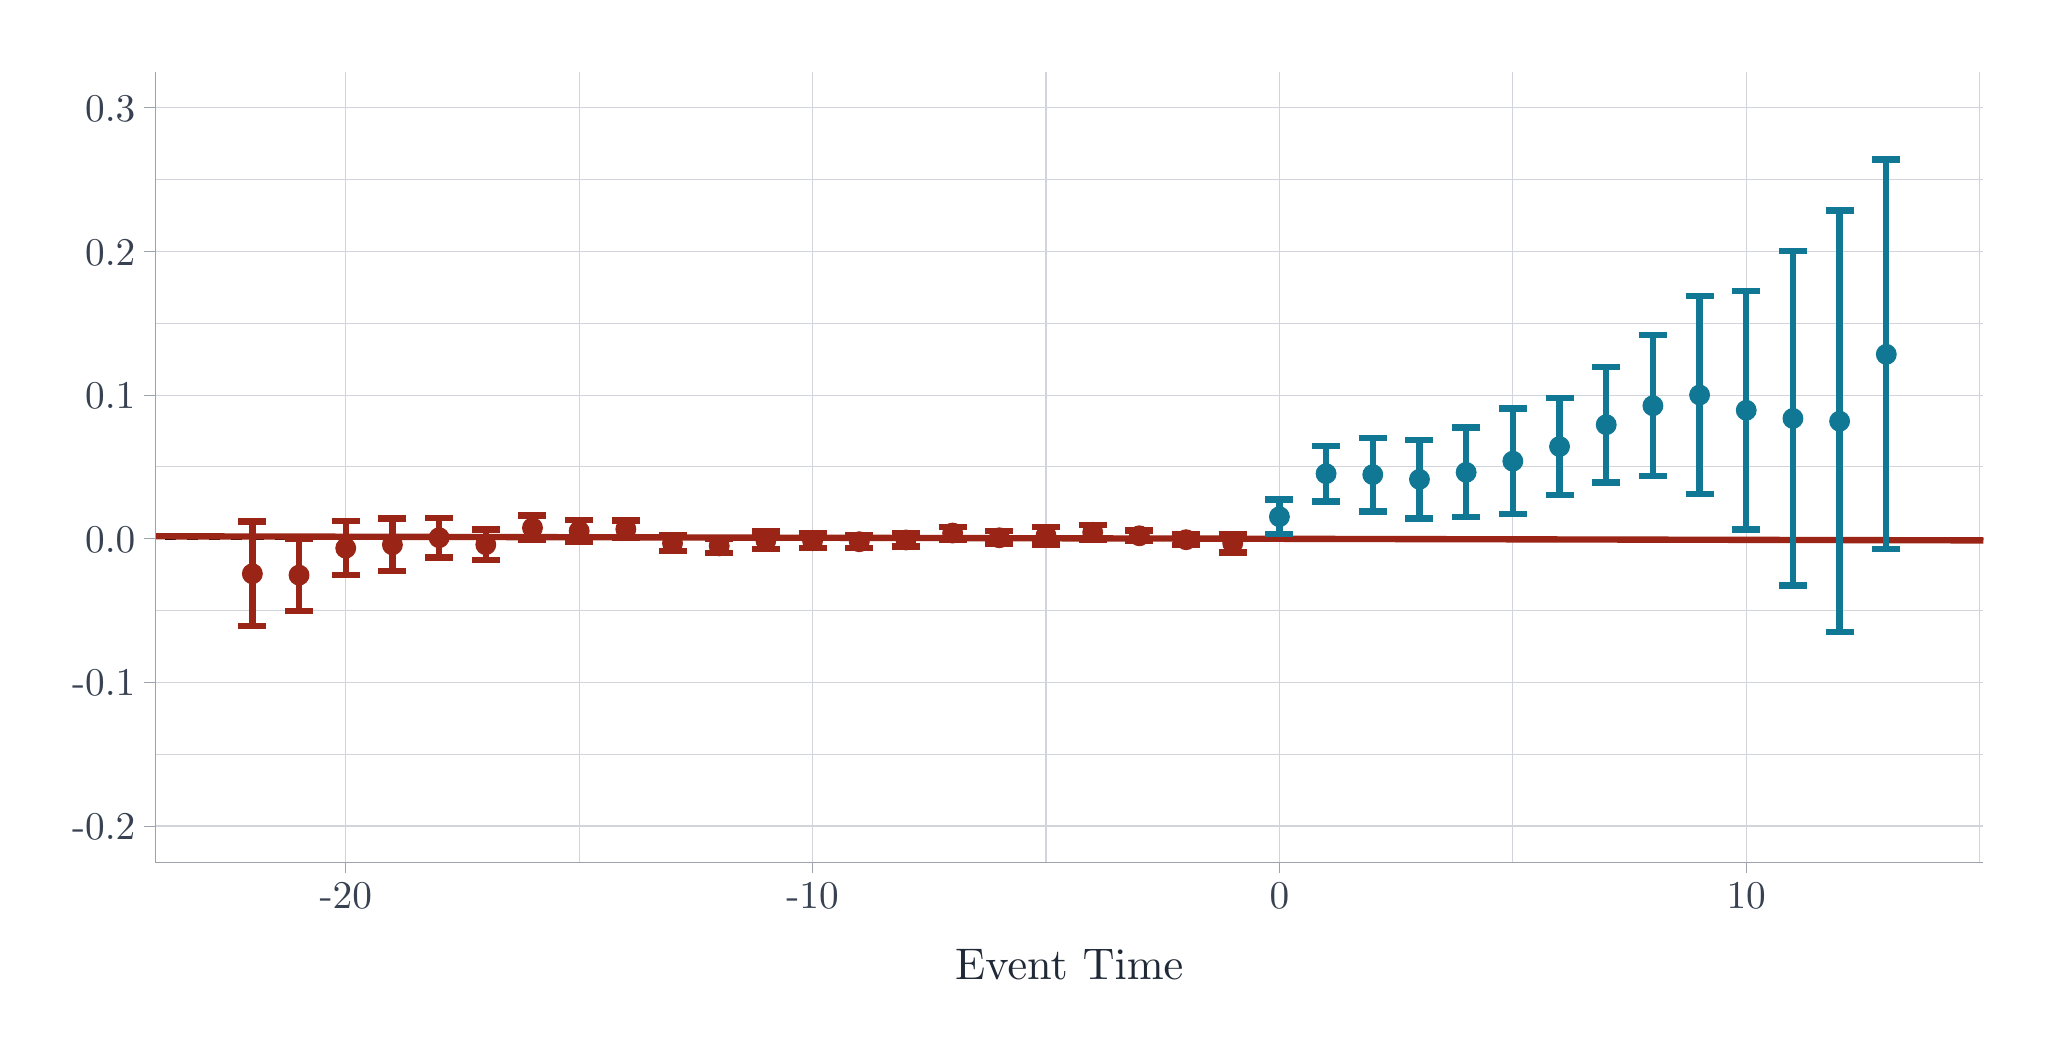
\begin{tikzpicture}[x=1pt,y=1pt]
\definecolor{fillColor}{RGB}{255,255,255}
\path[use as bounding box,fill=fillColor] (0,0) rectangle (722.70,361.35);
\begin{scope}
\path[clip] (  0.00,  0.00) rectangle (722.70,361.35);
\definecolor{drawColor}{RGB}{255,255,255}

\path[draw=drawColor,line width= 0.8pt,line join=round,line cap=round,fill=fillColor] (  0.00,  0.00) rectangle (722.70,361.35);
\end{scope}
\begin{scope}
\path[clip] ( 46.10, 59.89) rectangle (706.70,345.35);
\definecolor{drawColor}{RGB}{255,255,255}
\definecolor{fillColor}{RGB}{255,255,255}

\path[draw=drawColor,line width= 0.8pt,line join=round,line cap=round,fill=fillColor] ( 46.10, 59.89) rectangle (706.70,345.35);
\definecolor{drawColor}{RGB}{209,213,219}

\path[draw=drawColor,line width= 0.4pt,line join=round] ( 46.10, 98.81) --
	(706.70, 98.81);

\path[draw=drawColor,line width= 0.4pt,line join=round] ( 46.10,150.72) --
	(706.70,150.72);

\path[draw=drawColor,line width= 0.4pt,line join=round] ( 46.10,202.62) --
	(706.70,202.62);

\path[draw=drawColor,line width= 0.4pt,line join=round] ( 46.10,254.52) --
	(706.70,254.52);

\path[draw=drawColor,line width= 0.4pt,line join=round] ( 46.10,306.42) --
	(706.70,306.42);

\path[draw=drawColor,line width= 0.4pt,line join=round] (199.28, 59.89) --
	(199.28,345.35);

\path[draw=drawColor,line width= 0.4pt,line join=round] (367.97, 59.89) --
	(367.97,345.35);

\path[draw=drawColor,line width= 0.4pt,line join=round] (536.66, 59.89) --
	(536.66,345.35);

\path[draw=drawColor,line width= 0.4pt,line join=round] (705.35, 59.89) --
	(705.35,345.35);

\path[draw=drawColor,line width= 0.4pt,line join=round] ( 46.10, 72.86) --
	(706.70, 72.86);

\path[draw=drawColor,line width= 0.4pt,line join=round] ( 46.10,124.77) --
	(706.70,124.77);

\path[draw=drawColor,line width= 0.4pt,line join=round] ( 46.10,176.67) --
	(706.70,176.67);

\path[draw=drawColor,line width= 0.4pt,line join=round] ( 46.10,228.57) --
	(706.70,228.57);

\path[draw=drawColor,line width= 0.4pt,line join=round] ( 46.10,280.47) --
	(706.70,280.47);

\path[draw=drawColor,line width= 0.4pt,line join=round] ( 46.10,332.37) --
	(706.70,332.37);

\path[draw=drawColor,line width= 0.4pt,line join=round] (114.93, 59.89) --
	(114.93,345.35);

\path[draw=drawColor,line width= 0.4pt,line join=round] (283.62, 59.89) --
	(283.62,345.35);

\path[draw=drawColor,line width= 0.4pt,line join=round] (452.31, 59.89) --
	(452.31,345.35);

\path[draw=drawColor,line width= 0.4pt,line join=round] (621.00, 59.89) --
	(621.00,345.35);
\definecolor{drawColor}{RGB}{0,0,0}

\path[draw=drawColor,line width= 0.9pt,dash pattern=on 4pt off 4pt ,line join=round] (-614.49,176.67) -- (1367.30,176.67);
\definecolor{drawColor}{RGB}{154,36,21}

\path[draw=drawColor,line width= 2.3pt,line join=round] (-614.49,179.05) -- (1367.30,174.59);
\definecolor{fillColor}{RGB}{154,36,21}

\path[draw=drawColor,line width= 0.4pt,line join=round,line cap=round,fill=fillColor] ( 81.19,164.02) circle (  3.57);

\path[draw=drawColor,line width= 0.4pt,line join=round,line cap=round,fill=fillColor] ( 98.06,163.53) circle (  3.57);

\path[draw=drawColor,line width= 0.4pt,line join=round,line cap=round,fill=fillColor] (114.93,173.28) circle (  3.57);

\path[draw=drawColor,line width= 0.4pt,line join=round,line cap=round,fill=fillColor] (131.80,174.48) circle (  3.57);

\path[draw=drawColor,line width= 0.4pt,line join=round,line cap=round,fill=fillColor] (148.67,177.05) circle (  3.57);

\path[draw=drawColor,line width= 0.4pt,line join=round,line cap=round,fill=fillColor] (165.54,174.53) circle (  3.57);

\path[draw=drawColor,line width= 0.4pt,line join=round,line cap=round,fill=fillColor] (182.41,180.62) circle (  3.57);

\path[draw=drawColor,line width= 0.4pt,line join=round,line cap=round,fill=fillColor] (199.28,179.48) circle (  3.57);

\path[draw=drawColor,line width= 0.4pt,line join=round,line cap=round,fill=fillColor] (216.15,180.14) circle (  3.57);

\path[draw=drawColor,line width= 0.4pt,line join=round,line cap=round,fill=fillColor] (233.01,175.05) circle (  3.57);

\path[draw=drawColor,line width= 0.4pt,line join=round,line cap=round,fill=fillColor] (249.88,174.09) circle (  3.57);

\path[draw=drawColor,line width= 0.4pt,line join=round,line cap=round,fill=fillColor] (266.75,176.07) circle (  3.57);

\path[draw=drawColor,line width= 0.4pt,line join=round,line cap=round,fill=fillColor] (283.62,175.96) circle (  3.57);

\path[draw=drawColor,line width= 0.4pt,line join=round,line cap=round,fill=fillColor] (300.49,175.59) circle (  3.57);

\path[draw=drawColor,line width= 0.4pt,line join=round,line cap=round,fill=fillColor] (317.36,176.23) circle (  3.57);

\path[draw=drawColor,line width= 0.4pt,line join=round,line cap=round,fill=fillColor] (334.23,178.73) circle (  3.57);

\path[draw=drawColor,line width= 0.4pt,line join=round,line cap=round,fill=fillColor] (351.10,177.02) circle (  3.57);

\path[draw=drawColor,line width= 0.4pt,line join=round,line cap=round,fill=fillColor] (367.97,177.80) circle (  3.57);

\path[draw=drawColor,line width= 0.4pt,line join=round,line cap=round,fill=fillColor] (384.84,179.00) circle (  3.57);

\path[draw=drawColor,line width= 0.4pt,line join=round,line cap=round,fill=fillColor] (401.71,177.74) circle (  3.57);

\path[draw=drawColor,line width= 0.4pt,line join=round,line cap=round,fill=fillColor] (418.58,176.32) circle (  3.57);

\path[draw=drawColor,line width= 0.4pt,line join=round,line cap=round,fill=fillColor] (435.44,175.02) circle (  3.57);
\definecolor{drawColor}{RGB}{16,120,149}
\definecolor{fillColor}{RGB}{16,120,149}

\path[draw=drawColor,line width= 0.4pt,line join=round,line cap=round,fill=fillColor] (452.31,184.63) circle (  3.57);

\path[draw=drawColor,line width= 0.4pt,line join=round,line cap=round,fill=fillColor] (469.18,200.18) circle (  3.57);

\path[draw=drawColor,line width= 0.4pt,line join=round,line cap=round,fill=fillColor] (486.05,199.85) circle (  3.57);

\path[draw=drawColor,line width= 0.4pt,line join=round,line cap=round,fill=fillColor] (502.92,198.14) circle (  3.57);

\path[draw=drawColor,line width= 0.4pt,line join=round,line cap=round,fill=fillColor] (519.79,200.66) circle (  3.57);

\path[draw=drawColor,line width= 0.4pt,line join=round,line cap=round,fill=fillColor] (536.66,204.70) circle (  3.57);

\path[draw=drawColor,line width= 0.4pt,line join=round,line cap=round,fill=fillColor] (553.53,209.99) circle (  3.57);

\path[draw=drawColor,line width= 0.4pt,line join=round,line cap=round,fill=fillColor] (570.40,217.88) circle (  3.57);

\path[draw=drawColor,line width= 0.4pt,line join=round,line cap=round,fill=fillColor] (587.27,224.72) circle (  3.57);

\path[draw=drawColor,line width= 0.4pt,line join=round,line cap=round,fill=fillColor] (604.14,228.62) circle (  3.57);

\path[draw=drawColor,line width= 0.4pt,line join=round,line cap=round,fill=fillColor] (621.00,223.10) circle (  3.57);

\path[draw=drawColor,line width= 0.4pt,line join=round,line cap=round,fill=fillColor] (637.87,220.14) circle (  3.57);

\path[draw=drawColor,line width= 0.4pt,line join=round,line cap=round,fill=fillColor] (654.74,219.15) circle (  3.57);

\path[draw=drawColor,line width= 0.4pt,line join=round,line cap=round,fill=fillColor] (671.61,243.31) circle (  3.57);
\definecolor{drawColor}{RGB}{154,36,21}

\path[draw=drawColor,line width= 2.3pt,line join=round] ( 76.13,182.92) --
	( 86.25,182.92);

\path[draw=drawColor,line width= 2.3pt,line join=round] ( 81.19,182.92) --
	( 81.19,145.12);

\path[draw=drawColor,line width= 2.3pt,line join=round] ( 76.13,145.12) --
	( 86.25,145.12);

\path[draw=drawColor,line width= 2.3pt,line join=round] ( 93.00,176.48) --
	(103.12,176.48);

\path[draw=drawColor,line width= 2.3pt,line join=round] ( 98.06,176.48) --
	( 98.06,150.59);

\path[draw=drawColor,line width= 2.3pt,line join=round] ( 93.00,150.59) --
	(103.12,150.59);

\path[draw=drawColor,line width= 2.3pt,line join=round] (109.87,183.00) --
	(119.99,183.00);

\path[draw=drawColor,line width= 2.3pt,line join=round] (114.93,183.00) --
	(114.93,163.55);

\path[draw=drawColor,line width= 2.3pt,line join=round] (109.87,163.55) --
	(119.99,163.55);

\path[draw=drawColor,line width= 2.3pt,line join=round] (126.74,183.93) --
	(136.86,183.93);

\path[draw=drawColor,line width= 2.3pt,line join=round] (131.80,183.93) --
	(131.80,165.03);

\path[draw=drawColor,line width= 2.3pt,line join=round] (126.74,165.03) --
	(136.86,165.03);

\path[draw=drawColor,line width= 2.3pt,line join=round] (143.61,184.23) --
	(153.73,184.23);

\path[draw=drawColor,line width= 2.3pt,line join=round] (148.67,184.23) --
	(148.67,169.86);

\path[draw=drawColor,line width= 2.3pt,line join=round] (143.61,169.86) --
	(153.73,169.86);

\path[draw=drawColor,line width= 2.3pt,line join=round] (160.48,180.03) --
	(170.60,180.03);

\path[draw=drawColor,line width= 2.3pt,line join=round] (165.54,180.03) --
	(165.54,169.03);

\path[draw=drawColor,line width= 2.3pt,line join=round] (160.48,169.03) --
	(170.60,169.03);

\path[draw=drawColor,line width= 2.3pt,line join=round] (177.35,185.05) --
	(187.47,185.05);

\path[draw=drawColor,line width= 2.3pt,line join=round] (182.41,185.05) --
	(182.41,176.20);

\path[draw=drawColor,line width= 2.3pt,line join=round] (177.35,176.20) --
	(187.47,176.20);

\path[draw=drawColor,line width= 2.3pt,line join=round] (194.22,183.41) --
	(204.34,183.41);

\path[draw=drawColor,line width= 2.3pt,line join=round] (199.28,183.41) --
	(199.28,175.56);

\path[draw=drawColor,line width= 2.3pt,line join=round] (194.22,175.56) --
	(204.34,175.56);

\path[draw=drawColor,line width= 2.3pt,line join=round] (211.08,183.32) --
	(221.21,183.32);

\path[draw=drawColor,line width= 2.3pt,line join=round] (216.15,183.32) --
	(216.15,176.96);

\path[draw=drawColor,line width= 2.3pt,line join=round] (211.08,176.96) --
	(221.21,176.96);

\path[draw=drawColor,line width= 2.3pt,line join=round] (227.95,177.91) --
	(238.08,177.91);

\path[draw=drawColor,line width= 2.3pt,line join=round] (233.01,177.91) --
	(233.01,172.20);

\path[draw=drawColor,line width= 2.3pt,line join=round] (227.95,172.20) --
	(238.08,172.20);

\path[draw=drawColor,line width= 2.3pt,line join=round] (244.82,176.55) --
	(254.94,176.55);

\path[draw=drawColor,line width= 2.3pt,line join=round] (249.88,176.55) --
	(249.88,171.62);

\path[draw=drawColor,line width= 2.3pt,line join=round] (244.82,171.62) --
	(254.94,171.62);

\path[draw=drawColor,line width= 2.3pt,line join=round] (261.69,179.23) --
	(271.81,179.23);

\path[draw=drawColor,line width= 2.3pt,line join=round] (266.75,179.23) --
	(266.75,172.92);

\path[draw=drawColor,line width= 2.3pt,line join=round] (261.69,172.92) --
	(271.81,172.92);

\path[draw=drawColor,line width= 2.3pt,line join=round] (278.56,178.68) --
	(288.68,178.68);

\path[draw=drawColor,line width= 2.3pt,line join=round] (283.62,178.68) --
	(283.62,173.23);

\path[draw=drawColor,line width= 2.3pt,line join=round] (278.56,173.23) --
	(288.68,173.23);

\path[draw=drawColor,line width= 2.3pt,line join=round] (295.43,177.81) --
	(305.55,177.81);

\path[draw=drawColor,line width= 2.3pt,line join=round] (300.49,177.81) --
	(300.49,173.38);

\path[draw=drawColor,line width= 2.3pt,line join=round] (295.43,173.38) --
	(305.55,173.38);

\path[draw=drawColor,line width= 2.3pt,line join=round] (312.30,178.56) --
	(322.42,178.56);

\path[draw=drawColor,line width= 2.3pt,line join=round] (317.36,178.56) --
	(317.36,173.89);

\path[draw=drawColor,line width= 2.3pt,line join=round] (312.30,173.89) --
	(322.42,173.89);

\path[draw=drawColor,line width= 2.3pt,line join=round] (329.17,181.02) --
	(339.29,181.02);

\path[draw=drawColor,line width= 2.3pt,line join=round] (334.23,181.02) --
	(334.23,176.44);

\path[draw=drawColor,line width= 2.3pt,line join=round] (329.17,176.44) --
	(339.29,176.44);

\path[draw=drawColor,line width= 2.3pt,line join=round] (346.04,179.36) --
	(356.16,179.36);

\path[draw=drawColor,line width= 2.3pt,line join=round] (351.10,179.36) --
	(351.10,174.67);

\path[draw=drawColor,line width= 2.3pt,line join=round] (346.04,174.67) --
	(356.16,174.67);

\path[draw=drawColor,line width= 2.3pt,line join=round] (362.91,180.95) --
	(373.03,180.95);

\path[draw=drawColor,line width= 2.3pt,line join=round] (367.97,180.95) --
	(367.97,174.65);

\path[draw=drawColor,line width= 2.3pt,line join=round] (362.91,174.65) --
	(373.03,174.65);

\path[draw=drawColor,line width= 2.3pt,line join=round] (379.78,181.63) --
	(389.90,181.63);

\path[draw=drawColor,line width= 2.3pt,line join=round] (384.84,181.63) --
	(384.84,176.36);

\path[draw=drawColor,line width= 2.3pt,line join=round] (379.78,176.36) --
	(389.90,176.36);

\path[draw=drawColor,line width= 2.3pt,line join=round] (396.65,179.59) --
	(406.77,179.59);

\path[draw=drawColor,line width= 2.3pt,line join=round] (401.71,179.59) --
	(401.71,175.89);

\path[draw=drawColor,line width= 2.3pt,line join=round] (396.65,175.89) --
	(406.77,175.89);

\path[draw=drawColor,line width= 2.3pt,line join=round] (413.51,178.35) --
	(423.64,178.35);

\path[draw=drawColor,line width= 2.3pt,line join=round] (418.58,178.35) --
	(418.58,174.30);

\path[draw=drawColor,line width= 2.3pt,line join=round] (413.51,174.30) --
	(423.64,174.30);

\path[draw=drawColor,line width= 2.3pt,line join=round] (430.38,178.30) --
	(440.50,178.30);

\path[draw=drawColor,line width= 2.3pt,line join=round] (435.44,178.30) --
	(435.44,171.74);

\path[draw=drawColor,line width= 2.3pt,line join=round] (430.38,171.74) --
	(440.50,171.74);
\definecolor{drawColor}{RGB}{16,120,149}

\path[draw=drawColor,line width= 2.3pt,line join=round] (447.25,190.82) --
	(457.37,190.82);

\path[draw=drawColor,line width= 2.3pt,line join=round] (452.31,190.82) --
	(452.31,178.45);

\path[draw=drawColor,line width= 2.3pt,line join=round] (447.25,178.45) --
	(457.37,178.45);

\path[draw=drawColor,line width= 2.3pt,line join=round] (464.12,210.19) --
	(474.24,210.19);

\path[draw=drawColor,line width= 2.3pt,line join=round] (469.18,210.19) --
	(469.18,190.17);

\path[draw=drawColor,line width= 2.3pt,line join=round] (464.12,190.17) --
	(474.24,190.17);

\path[draw=drawColor,line width= 2.3pt,line join=round] (480.99,213.15) --
	(491.11,213.15);

\path[draw=drawColor,line width= 2.3pt,line join=round] (486.05,213.15) --
	(486.05,186.56);

\path[draw=drawColor,line width= 2.3pt,line join=round] (480.99,186.56) --
	(491.11,186.56);

\path[draw=drawColor,line width= 2.3pt,line join=round] (497.86,212.25) --
	(507.98,212.25);

\path[draw=drawColor,line width= 2.3pt,line join=round] (502.92,212.25) --
	(502.92,184.03);

\path[draw=drawColor,line width= 2.3pt,line join=round] (497.86,184.03) --
	(507.98,184.03);

\path[draw=drawColor,line width= 2.3pt,line join=round] (514.73,216.89) --
	(524.85,216.89);

\path[draw=drawColor,line width= 2.3pt,line join=round] (519.79,216.89) --
	(519.79,184.43);

\path[draw=drawColor,line width= 2.3pt,line join=round] (514.73,184.43) --
	(524.85,184.43);

\path[draw=drawColor,line width= 2.3pt,line join=round] (531.60,223.77) --
	(541.72,223.77);

\path[draw=drawColor,line width= 2.3pt,line join=round] (536.66,223.77) --
	(536.66,185.63);

\path[draw=drawColor,line width= 2.3pt,line join=round] (531.60,185.63) --
	(541.72,185.63);

\path[draw=drawColor,line width= 2.3pt,line join=round] (548.47,227.46) --
	(558.59,227.46);

\path[draw=drawColor,line width= 2.3pt,line join=round] (553.53,227.46) --
	(553.53,192.53);

\path[draw=drawColor,line width= 2.3pt,line join=round] (548.47,192.53) --
	(558.59,192.53);

\path[draw=drawColor,line width= 2.3pt,line join=round] (565.34,238.72) --
	(575.46,238.72);

\path[draw=drawColor,line width= 2.3pt,line join=round] (570.40,238.72) --
	(570.40,197.04);

\path[draw=drawColor,line width= 2.3pt,line join=round] (565.34,197.04) --
	(575.46,197.04);

\path[draw=drawColor,line width= 2.3pt,line join=round] (582.21,250.19) --
	(592.33,250.19);

\path[draw=drawColor,line width= 2.3pt,line join=round] (587.27,250.19) --
	(587.27,199.24);

\path[draw=drawColor,line width= 2.3pt,line join=round] (582.21,199.24) --
	(592.33,199.24);

\path[draw=drawColor,line width= 2.3pt,line join=round] (599.07,264.31) --
	(609.20,264.31);

\path[draw=drawColor,line width= 2.3pt,line join=round] (604.14,264.31) --
	(604.14,192.92);

\path[draw=drawColor,line width= 2.3pt,line join=round] (599.07,192.92) --
	(609.20,192.92);

\path[draw=drawColor,line width= 2.3pt,line join=round] (615.94,266.21) --
	(626.07,266.21);

\path[draw=drawColor,line width= 2.3pt,line join=round] (621.00,266.21) --
	(621.00,180.00);

\path[draw=drawColor,line width= 2.3pt,line join=round] (615.94,180.00) --
	(626.07,180.00);

\path[draw=drawColor,line width= 2.3pt,line join=round] (632.81,280.54) --
	(642.93,280.54);

\path[draw=drawColor,line width= 2.3pt,line join=round] (637.87,280.54) --
	(637.87,159.74);

\path[draw=drawColor,line width= 2.3pt,line join=round] (632.81,159.74) --
	(642.93,159.74);

\path[draw=drawColor,line width= 2.3pt,line join=round] (649.68,295.26) --
	(659.80,295.26);

\path[draw=drawColor,line width= 2.3pt,line join=round] (654.74,295.26) --
	(654.74,143.04);

\path[draw=drawColor,line width= 2.3pt,line join=round] (649.68,143.04) --
	(659.80,143.04);

\path[draw=drawColor,line width= 2.3pt,line join=round] (666.55,313.73) --
	(676.67,313.73);

\path[draw=drawColor,line width= 2.3pt,line join=round] (671.61,313.73) --
	(671.61,172.90);

\path[draw=drawColor,line width= 2.3pt,line join=round] (666.55,172.90) --
	(676.67,172.90);
\end{scope}
\begin{scope}
\path[clip] (  0.00,  0.00) rectangle (722.70,361.35);
\definecolor{drawColor}{RGB}{156,163,175}

\path[draw=drawColor,line width= 0.3pt,line join=round] ( 46.10, 59.89) --
	( 46.10,345.35);
\end{scope}
\begin{scope}
\path[clip] (  0.00,  0.00) rectangle (722.70,361.35);
\definecolor{drawColor}{RGB}{55,65,81}

\node[text=drawColor,anchor=base east,inner sep=0pt, outer sep=0pt, scale=  1.42] at ( 38.90, 67.97) {-0.2};

\node[text=drawColor,anchor=base east,inner sep=0pt, outer sep=0pt, scale=  1.42] at ( 38.90,119.87) {-0.1};

\node[text=drawColor,anchor=base east,inner sep=0pt, outer sep=0pt, scale=  1.42] at ( 38.90,171.77) {0.0};

\node[text=drawColor,anchor=base east,inner sep=0pt, outer sep=0pt, scale=  1.42] at ( 38.90,223.67) {0.1};

\node[text=drawColor,anchor=base east,inner sep=0pt, outer sep=0pt, scale=  1.42] at ( 38.90,275.58) {0.2};

\node[text=drawColor,anchor=base east,inner sep=0pt, outer sep=0pt, scale=  1.42] at ( 38.90,327.48) {0.3};
\end{scope}
\begin{scope}
\path[clip] (  0.00,  0.00) rectangle (722.70,361.35);
\definecolor{drawColor}{RGB}{156,163,175}

\path[draw=drawColor,line width= 0.3pt,line join=round] ( 42.10, 72.86) --
	( 46.10, 72.86);

\path[draw=drawColor,line width= 0.3pt,line join=round] ( 42.10,124.77) --
	( 46.10,124.77);

\path[draw=drawColor,line width= 0.3pt,line join=round] ( 42.10,176.67) --
	( 46.10,176.67);

\path[draw=drawColor,line width= 0.3pt,line join=round] ( 42.10,228.57) --
	( 46.10,228.57);

\path[draw=drawColor,line width= 0.3pt,line join=round] ( 42.10,280.47) --
	( 46.10,280.47);

\path[draw=drawColor,line width= 0.3pt,line join=round] ( 42.10,332.37) --
	( 46.10,332.37);
\end{scope}
\begin{scope}
\path[clip] (  0.00,  0.00) rectangle (722.70,361.35);
\definecolor{drawColor}{RGB}{156,163,175}

\path[draw=drawColor,line width= 0.3pt,line join=round] ( 46.10, 59.89) --
	(706.70, 59.89);
\end{scope}
\begin{scope}
\path[clip] (  0.00,  0.00) rectangle (722.70,361.35);
\definecolor{drawColor}{RGB}{156,163,175}

\path[draw=drawColor,line width= 0.3pt,line join=round] (114.93, 55.89) --
	(114.93, 59.89);

\path[draw=drawColor,line width= 0.3pt,line join=round] (283.62, 55.89) --
	(283.62, 59.89);

\path[draw=drawColor,line width= 0.3pt,line join=round] (452.31, 55.89) --
	(452.31, 59.89);

\path[draw=drawColor,line width= 0.3pt,line join=round] (621.00, 55.89) --
	(621.00, 59.89);
\end{scope}
\begin{scope}
\path[clip] (  0.00,  0.00) rectangle (722.70,361.35);
\definecolor{drawColor}{RGB}{55,65,81}

\node[text=drawColor,anchor=base,inner sep=0pt, outer sep=0pt, scale=  1.42] at (114.93, 42.89) {-20};

\node[text=drawColor,anchor=base,inner sep=0pt, outer sep=0pt, scale=  1.42] at (283.62, 42.89) {-10};

\node[text=drawColor,anchor=base,inner sep=0pt, outer sep=0pt, scale=  1.42] at (452.31, 42.89) {0};

\node[text=drawColor,anchor=base,inner sep=0pt, outer sep=0pt, scale=  1.42] at (621.00, 42.89) {10};
\end{scope}
\begin{scope}
\path[clip] (  0.00,  0.00) rectangle (722.70,361.35);
\definecolor{drawColor}{RGB}{31,41,55}

\node[text=drawColor,anchor=base,inner sep=0pt, outer sep=0pt, scale=  1.60] at (376.40, 17.56) {Event Time};
\end{scope}
\end{tikzpicture}
